% "{'classe':('PSI'),'chapitre':'dyn_pfd_cf','type':('application'),'titre':'Micromoteur de modélisme', 'source':'Équipe PT La Martinière Monplaisir','comp':('C1-05','C2-09'),'corrige':True}"
%\setchapterimage{bandeau}
\chapter*{Application \arabic{cptApplication} \\ 
Chaîne fermée -- Micromoteur de modélisme  \ifnormal $\star$ \else \fi \ifdifficile $\star\star$ \else \fi \iftdifficile $\star\star\star$ \else \fi
-- \ifprof Corrigé \else Sujet \fi}
\addcontentsline{toc}{section}{Application \arabic{cptApplication} : Chaîne fermée -- Micromoteur de modélisme  \ifnormal $\star$ \else \fi \ifdifficile $\star\star$ \else \fi \iftdifficile $\star\star\star$ \else \fi -- \ifprof Corrigé \else Sujet \fi}

\iflivret \stepcounter{cptApplication} \else
\ifprof  \stepcounter{cptApplication} \else \fi
\fi

\setcounter{question}{0}
\marginnote{Équipe PT La Martinière Monplaisir.}
\marginnote[1cm]{
\UPSTIcompetence[2]{C1-05}
\UPSTIcompetence[2]{C2-09}
}
\begin{marginfigure}
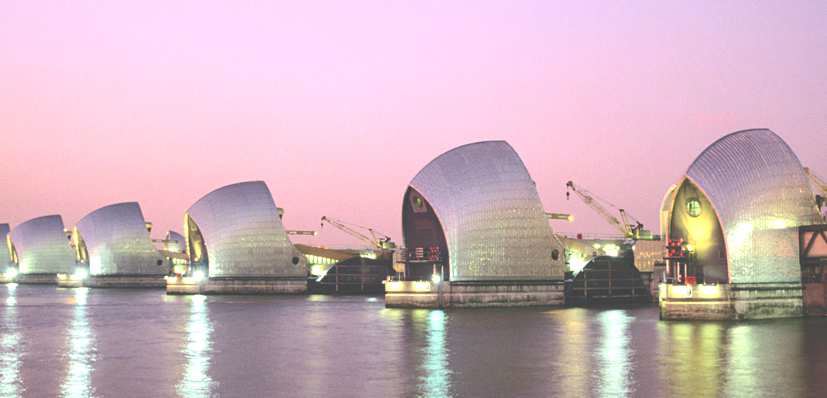
\includegraphics[width=\linewidth]{fig_00}
\end{marginfigure}


\subsection*{Mise en situation}
\ifprof
\else
Les figures et le schéma ci-dessous représentent un micromoteur à combustion interne de modèle réduit. Du point de vue cinématique, il est basé sur un système bielle manivelle \textbf{(2,1)}, associé à un piston \textbf{(3)}, animé d’un mouvement de translation rectiligne alternatif. 

\begin{marginfigure}
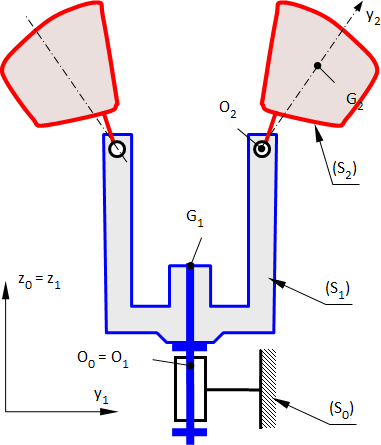
\includegraphics[width=\linewidth]{fig_02}
\end{marginfigure}


On note : 
\begin{itemize}
\item $\vect{AB}=e\vect{x_1}$, $\vect{BC}=L_2\vect{y_2}$, $\vect{AC}=\lambda_3\vect{y_0}$;
\item $\vect{HG_1}=a_1\vect{x_1}$, $\vect{BG_2}=a_2\vect{y_2}$, $\vect{CG_3}=a_3\vect{y_0}$;
\item $\angl{x_0}{x_1}=\angl{y_0}{y_1}=\theta_1$, $\angl{x_0}{x_2}=\angl{y_0}{y_2}=\theta_2$; $\omega_{10}=\dot{\theta}_1$ et $\omega_{20}=\dot{\theta}_2$;
\item $m_1$, $m_2$ et $m_3$ les masses des trois pièces mobiles \textbf{(1)}, \textbf{(2)} et \textbf{(3)}.
\end{itemize}

On note $C_m \vect{z_0}$ le couple délivré par le moteur et $F_e \vect{y_0}$ la force exercée sur le piston suite à l'explosion du mélange air -- carburant. On néglige les effets de la pesanteur.
\fi

\question{Exprimer la relation liant la vitesse de rotation $\omega_{10}$ du vilebrequin \textbf{(1)} et la vitesse du piston \textbf{(3)}, notée $\dot{\lambda}=V_{3/0}$.}% Déterminer la vitesse et l'accélération du centre d'inertie de la bielle \textbf{(2)} par rapport à \textbf{(0)}.}

\ifprof
\begin{corrige}
On réalise une fermeture géométrique dans le triangle $ABC$ et on a : 
$\vect{AB}+\vect{BC}+\vect{CA}=\vect{0}$ $\Leftrightarrow e\vect{x_1}+L_2\vect{x_2}-\lambda_3 \vect{y_0}$ $\Leftrightarrow e\left( \cos \theta_1 \vect{x_0}+\sin \theta_1 \vect{y_0} \right)+L_2\left( \cos \theta_2 \vect{x_0}+\sin \theta_2 \vect{y_0} \right)-\lambda_3 \vect{y_0} = \vect{0}$. 
On a donc : 
$\left\{
\begin{array}{l}
e\cos \theta_1 +L_2 \cos \theta_2 = 0 \\
e\sin \theta_1 + L_2 \sin \theta_2 -\lambda_3 = 0
\end{array}
\right.$
$\Leftrightarrow \left\{
\begin{array}{l}
L_2 \cos \theta_2 = -e\cos \theta_1  \\
L_2 \sin \theta_2  = \lambda_3-e\sin \theta_1
\end{array}
\right.
$
Au final, $L_2^2 = e^2\cos^2 \theta_1 + \left(\lambda_3-e\sin \theta_1\right)^2$
$\Leftrightarrow L_2^2 - e^2\cos^2 \theta_1 = \left(\lambda_3-e\sin \theta_1\right)^2$

$\Rightarrow \sqrt{L_2^2 - e^2\cos^2 \theta_1} = \lambda_3-e\sin \theta_1$
$ \Rightarrow \lambda_3 = \sqrt{L_2^2 - e^2\cos^2 \theta_1}+e\sin \theta_1$.

\end{corrige}
\else
\fi

\ifprof

\else
Dans la perspective d’une étude dynamique, on se propose d’évaluer les caractéristiques de masse et inertie des trois pièces mobiles, ainsi que leurs propriétés cinétiques.

On note $\inertie{H}{1}=\matinertie{A_1}{B_1}{C_1}{-D_1}{-E_1}{-F_1}{\repere{H}{x_1}{y_1}{z_1}}$ la matrice d'inertie en $H$ de l'ensemble \{vilebrequin, hélice\} repéré~\textbf{(1)}. 
\fi

\question{En considérant que seul le plan $\left(H,\vect{x_1},\vect{z_1}\right)$ est le plan de symétrie, indiquer quelle(s) simplification(s) cela apporte à cette matrice d'inertie.} 

\ifprof
\begin{corrige}
On a donc une invariance suivant $\vect{y_1}$ et 
$\inertie{H}{1}=\matinertie{A_1}{B_1}{C_1}{0}{-E_1}{0}{\repere{H}{x_1}{y_1}{z_1}}$
\end{corrige}
\else
\fi

%
%\subparagraph{}
%\textit{Définir la forme de la matrice d’inertie de la bielle \textbf{(2)} et du piston \textbf{(3)} en précisant en quel point et dans quelle base elle est définie.}
%\ifprof
%\begin{corrige}
%De même $\inertie{G_2}{2}=\matinertie{A_2}{B_2}{C_2}{0}{-E_2}{0}{\repere{G_2}{x_2}{y_2}{z_2}}$ et 
%$\inertie{G_3}{3}=\matinertie{A_2}{B_2}{C_2}{0}{-E_2}{0}{\repere{G_3}{x_2}{y_2}{z_2}}$.
%\end{corrige}
%\else
%\fi


Par la suite on fait l'hypothèse que les matrices d'inertie $\inertie{A}{1}$, $\inertie{G_2}{2}$ et $\inertie{G_3}{3}$ sont diagonales. 

%\subparagraph{}
%\textit{Exprimer, pour chacune d’elles : son torseur cinétique et son torseur dynamique.}
\ifprof
\begin{corrige}
$H$ est un point fixe : 
\begin{itemize}
\item $\torseurci{1}{0}
=\torseurl{\vectrc{1}{0}=m_1\vectv{G_1}{1}{0}}{\vectmc{H}{1}{0}=\inertie{H}{1}\vecto{1}{0}}{H}
=\torseurl{\vect{0}}{C_1\dot{\theta}_1\vect{z_1}}{H}$
\item $\torseurdyn{1}{0}
=\torseurl{\vectrd{1}{0}=m_1\vectg{G_1}{1}{0}}{\vectmd{H}{1}{0}=\left[\dfrac{\dd \vectmd{H}{1}{0}}{\dd t}\right]_{\mathcal{R}_0}}{H}
=\torseurl{\vect{0}}{C_1\ddot{\theta}_1\vect{z_1}}{H}$
\end{itemize}


$G_3$ est le centre de gravité de 3. Le solide 3 est en translation par rapport à 0.
\begin{itemize}
\item $\torseurci{3}{0}
=\torseurl{\vectrc{3}{0}=m_3\vectv{G_3}{3}{0}}{\vectmc{G_3}{3}{0}}{G_3}
=\torseurl{m_3\dot{\lambda}_3\vect{y_0}}{\vect{0}}{G_3}$
\item $\torseurdyn{3}{0}
=\torseurl{\vectrd{3}{0}=m_1\vectg{G_3}{3}{0}}{\vectmd{G_3}{1}{0}=\left[\dfrac{\dd \vectmc{G_3}{3}{0}}{\dd t}\right]_{\mathcal{R}_0}}{G_3}
=\torseurl{m_3\ddot{\lambda}_3\vect{y_0}}{\vect{0}}{G_3}$
\end{itemize}

$G_2$ est le centre de gravité de 2.
\begin{itemize}
\item $\torseurci{2}{0}
=\torseurl{\vectrc{2}{0}=m_2\vectv{G_2}{2}{0}}{\vectmc{G_2}{2}{0}=\inertie{G_2}{2}\vecto{2}{0}}{G_2}
=\torseurl{ m_2 \left(\dot{\lambda}_3\vect{y_0}+a_2 \dot{\theta}_2\vect{x_2}\right) }{
C_2 \dot{\theta}_2 \vect{z_0}  }{G_2}$
\item $\torseurdyn{2}{0}
=\torseurl{\vectrd{2}{0}=m_2\vectg{G_2}{2}{0}}{\vectmd{G_2}{2}{0}=\left[\dfrac{\dd \vectmc{G_2}{2}{0}}{\dd t}\right]_{\mathcal{R}_0}}{G_2}
=\torseurl{ m_2 \left(\ddot{\lambda}_3\vect{y_0}+a_2 \ddot{\theta}_2\vect{x_2}+a_2 \dot{\theta}_2^2\vect{y_2}\right) }{C_2 \ddot{\theta}_2 \vect{z_0}  }{G_2}$
\end{itemize}

Détail des calculs.

\textbf{Calcul de  $\vectv{G_2}{2}{0}$.}

$ \vectv{G_2}{2}{0} = \vectv{G_2}{2}{3}+\vectv{G_2}{3}{0}$

$\vectv{G_2}{2}{3}=\vectv{C}{2}{3}+\vect{G_2C}\wedge \vecto{2}{3}=\vect{0}+a_2\vect{y_2}\wedge \dot{\theta}_2\vect{z_0}=a_2 \dot{\theta}_2\vect{x_2}$
$\quad$ 
$\vectv{G_2}{3}{0}=\dot{\lambda}_3\vect{y_0}$ 

$ \vectv{G_2}{2}{0}=\dot{\lambda}_3\vect{y_0}+a_2 \dot{\theta}_2\vect{x_2}$.

\textbf{Calcul de  $\vectg{G_2}{2}{0}$.}

$ \vectg{G_2}{2}{0}=\ddot{\lambda}_3\vect{y_0}+a_2 \ddot{\theta}_2\vect{x_2}+a_2 \dot{\theta}_2^2\vect{y_2}$.
\end{corrige}
\else
\fi

\question{Déterminer l'équation de mouvement par les théorèmes généraux.}
\ifprof
\begin{corrige} ~\\
\begin{itemize}
\item On isole \textbf{(1)}.
\item Bilan des actions mécaniques extérieures :
\begin{itemize}
\item Liaison pivot : $\torseurstat{T}{0}{1}=\torseurl{\vectf{0}{1}}{\vectm{A}{0}{1}}{A}$ avec $\vectm{A}{0}{1}\cdot\vect{z_0}=0$ (pas de frottement dans la liaison).
\item Liaison pivot : $\torseurstat{T}{2}{1}=\torseurl{\vectf{2}{1}}{\vectm{B}{2}{1}}{B}$ avec $\vectm{B}{2}{1}\cdot\vect{z_0}=0$ (pas de frottement dans la liaison).
Par ailleurs, $\vectm{A}{2}{1}\cdot\vect{z_0}=\vectm{B}{2}{1}\cdot\vect{z_0}+\left(\vect{AB}\wedge\vectf{2}{1}\right) \vect{z_0}=\left(e\vect{x_1}\wedge\left(X_{21}\vect{x_2}+Y_{21}\vect{y_2}\right)\right)\vect{z_0}$
$=\left(eX_{21}\vect{x_1}\wedge \vect{x_2}+ eY_{21} \vect{x_1}\wedge \vect{y_2}\right)\vect{z_0} $
$=eX_{21}\sin \left( \theta_2 - \theta_1\right)+ eY_{21} \cos \left( \theta_2 - \theta_1\right) $

\item Couple moteur : $\torseurstat{T}{0_m}{1}=\torseurl{\vect{0}}{C_m\vect{z_0}}{A}$.
\end{itemize}
\item On applique le TMD en $A$ en projection suivant $\vect{z}$ :
$$
eX_{21}\sin \left( \theta_2 - \theta_1\right)+ eY_{21} \cos \left( \theta_2 - \theta_1\right) + C_m=C_1\ddot{\theta}_1
$$
\end{itemize}

%\begin{itemize}
%\item On isole \textbf{(3)}.
%\item Bilan des actions mécaniques extérieures :
%\begin{itemize}
%\item Liaison glissière: $\torseurstat{T}{0}{3}=\torseurl{\vectf{0}{3}}{\vectm{A}{0}{3}}{A}$ avec $\vectf{0}{3}\cdot\vect{y_0}=0$ (pas de frottement dans la liaison).
%\item Liaison pivot : $\torseurstat{T}{2}{3}=\torseurl{\vectf{2}{3}}{\vectm{C}{2}{3}}{C}$ avec $\vectm{C}{2}{3}\cdot\vect{z_0}=0$ (pas de frottement dans la liaison).
%\item Force explosion: $\torseurstat{T}{0_e}{3}=\torseurl{F_y\vect{y}+F_z\vect{z}}{\vect{C_{exp}}}{C}$.
%\end{itemize}
%\item On applique le TMD en $C$ projection suivant $\vect{z_0}$ :
%$$
%F_y+Y_{23}=m_3\ddot{\lambda}_3
%$$
%\end{itemize}


\begin{itemize}
\item On isole \textbf{(2)}.
\item Bilan des actions mécaniques extérieures :
\begin{itemize}
\item Liaison pivot : $\torseurstat{T}{1}{2}=\torseurl{-\vectf{2}{1}}{-\vectm{B}{2}{1}}{B}$ avec $\vectm{B}{2}{1}\cdot\vect{z_0}=0$ (pas de frottement dans la liaison).
\item Liaison pivot : $\torseurstat{T}{3}{2}=\torseurl{-\vectf{2}{3}}{-\vectm{C}{2}{3}}{C}$ avec $\vectm{C}{2}{3}\cdot\vect{z_0}=0$ (pas de frottement dans la liaison).
\end{itemize}
\item On applique le TMD en $C$ en projection sur $\vect{z_0}$ :
%TRD
%$$
%-Y_{21}-Y_{23}=\left(m_2 \left(\ddot{\lambda}_3\vect{y_0}+a_2 \ddot{\theta}_2\vect{x_2}+a_2 \dot{\theta}_2^2\vect{y_2}\right)\right)\cdot\vect{y_0}. 
%$$
$$
- \vect{CB}\wedge\vectf{2}{1}\cdot \vect{z} = \vectmd{C}{2}{0}\cdot \vect{z}
\Longleftrightarrow 
L_2\vect{y_2} \wedge\left( X_{21}\vect{x_2}+ Y_{21}\vect{y_2}\right)\cdot \vect{z} = \left( \vectmd{G_2}{2}{0} + \vect{CG_2}\wedge m_2\vectg{G_2}{2}{0} \right)\cdot \vect{z}
$$

$$
\Longrightarrow 
-L_2 X_{21} = C_2\ddot{\theta}_2\left(  -a_2 \vect{y_2}\wedge \left(  m_2 \left(\ddot{\lambda}_3\vect{y_0}+a_2 \ddot{\theta}_2\vect{x_2}+a_2 \dot{\theta}_2^2\vect{y_2}\right)\right) \right)\cdot \vect{z}
$$
$$
\Longrightarrow 
-L_2 X_{21} = C_2\ddot{\theta}_2+a_2 m_2 \left(\ddot{\lambda}_3 \sin\theta_2-  a_2 \ddot{\theta}_2\vect{z_2}\right)
$$
\end{itemize}



\begin{itemize}
\item On isole \textbf{(2+3)}.
\item Bilan des actions mécaniques extérieures :
\begin{itemize}
\item Liaison glissière: $\torseurstat{T}{0}{3}=\torseurl{\vectf{0}{3}}{\vectm{A}{0}{3}}{A}$ avec $\vectf{0}{3}\cdot\vect{y_0}=0$ (pas de frottement dans la liaison).
\item Liaison pivot : $\torseurstat{T}{1}{2}=\torseurl{-\vectf{2}{1}}{-\vectm{B}{2}{1}}{B}$ avec $\vectm{B}{2}{1}\cdot\vect{z_0}=0$ (pas de frottement dans la liaison).
\item Force explosion: $\torseurstat{T}{0_e}{3}=\torseurl{F_y\vect{y}+F_z\vect{z}}{\vect{C_{exp}}}{C}$.
\end{itemize}
\item On applique le TRD en projection sur $\vect{y_0}$ :
$$
F_y-Y_{21}=m_3\ddot{\lambda}_3+\left(  m_2 \left(\ddot{\lambda}_3\vect{y_0}+a_2 \ddot{\theta}_2\vect{x_2}+a_2 \dot{\theta}_2^2\vect{y_2}\right)\right)\cdot \vect{y_0}
$$

$$
\Longleftrightarrow
F_y-Y_{21}=m_3\ddot{\lambda}_3+\left(  m_2 \left(\ddot{\lambda}_3+a_2 \ddot{\theta}_2 \sin \theta_2+a_2 \dot{\theta}_2^2\cos\theta_2\right)\right)
$$
\end{itemize}
\end{corrige}
\else
\fi




\ifprof
\else
\begin{center}
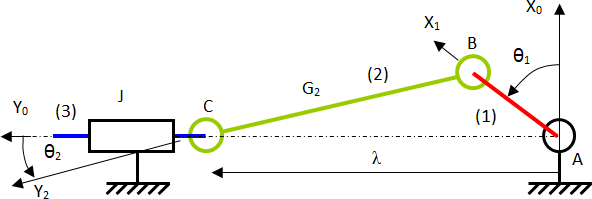
\includegraphics[width=.7\linewidth]{fig_03}
\end{center}
\fi

